% =============================================================================
% Overleaf
%   Zip the repo so paper/ and figures/ stay in place.
%   New Project -> Upload Project.
%   Main document: paper/main.tex
%   Compiler: pdfLaTeX. Recompile twice so the bibliography shows up.
%   Put your real department, college, city, and email in the author block
%   before you submit. Leave it blank rather than guessing.
% =============================================================================

\documentclass[conference]{IEEEtran}

\usepackage{cite}
\usepackage{amsmath,amssymb}
\usepackage{graphicx}
\usepackage{booktabs}
\usepackage{url}
\graphicspath{{../figures/}{figures/}}

\begin{document}

\title{Ridge, Lasso, and Elastic Net Do Not Beat\\
Least Squares on Community Violent Crime}

\author{
\IEEEauthorblockN{Himanshu}
\IEEEauthorblockA{
% Fill these in. Do not leave the placeholders in a submission.
\textit{Add department and institution}\\
Add city, country\\
email@institution.edu}
}

\maketitle

\begin{abstract}
We compare ordinary least squares, ridge regression, the lasso, and elastic net on the UCI Communities and Crime data.
The file has 1{,}994 communities.
After identifiers and mostly blank police-survey fields are removed, 100 predictors remain.
The target is the 1995 violent-crime rate, already scaled to the interval from 0 to 1.
On a held-out 20\% of communities (seed 42) the test $R^{2}$ values are 0.638, 0.640, 0.642, and 0.642.
Root-mean-square error drops from 0.221, which is what we get by predicting the training mean, to about 0.131.
Five further splits give mean test $R^{2}$ of 0.652, 0.654, 0.652, and 0.652.
The gap between models is about 0.003.
The gap between splits is about 0.03.
Elastic net chooses an $\ell_1$ ratio of 0.1, keeps 81 coefficients, and does not win any of the five splits.
The penalties still matter for reading the fit.
Forty-nine predictor pairs correlate at 0.90 or above, and least squares puts large weights of opposite sign on some of those pairs.
We treat every coefficient as a partial association.
The study does not estimate what would happen if a community changed one of these columns.
\end{abstract}

\begin{IEEEkeywords}
communities and crime, least squares, ridge regression, lasso, elastic net, multicollinearity
\end{IEEEkeywords}

\section{Introduction}
We started from a simple question.
If the census columns are left as they are, with the near-duplicate measures still in the table, does a penalty predict the violent-crime rate better than ordinary least squares?
Ridge, the lasso, and elastic net are the usual answers when a design is collinear \cite{hoerl1970,tibshirani1996,zou2005}.
We wanted the comparison on one public file, with the penalty chosen only from the training communities, and with more than one split.

The file is the UCI Communities and Crime extract \cite{redmond2002,uci2009}.
It was released so that people could try attribute weighting on a real social table.
The target is \texttt{ViolentCrimesPerPop}.
It combines 1995 counts of murder, rape, robbery, and assault with population, and the archive already maps the numeric columns onto roughly 0 to 1.

Two recent papers fit a lasso on this collection and then discuss the nonzero coefficients as the factors behind the crime rate \cite{dai2024,wei2025}.
A 2023 conference paper on linear, ridge, and lasso crime models reports an average predictive accuracy of 94\% \cite{david2023}.
We cite that figure as theirs.
It is not the holdout $R^{2}$ we compute here, which is about 0.64.
A model can be useful at that level and still leave a large share of the variance untouched.

Our result is easy to state.
All four models beat the mean by a wide margin, and they match each other closely enough that the split matters more than the penalty.
What changes is the coefficient vector.
Least squares uses near-copy columns to cancel one another.
The penalties shrink those weights or set them to zero.
That is a better description of the table.
It is still a description of a fit, and we do not read it as a cause.

\section{What other papers do with this file}
Redmond and Baveja built the source table from the 1990 Census, the 1990 LEMAS police survey, and the 1995 Uniform Crime Reports \cite{redmond2002}.
Communities that could not be matched, and communities with inconsistent rape figures, are absent from the public extract of 1{,}994 rows \cite{uci2009}.

Dai applies the lasso and highlights housing cost, education, and the share of teenagers in two-parent households \cite{dai2024}.
Wei also uses the lasso, removes race-coded columns, and reports family structure and housing \cite{wei2025}.
Both are short, readable equations.
Neither paper shows the unpenalized least-squares fit on the same rows, so a reader cannot see whether the penalty changed the predictions.
Kim and Park compare penalties inside a two-part model for crime counts \cite{kim2024}.
Their sample and their response are different from the single normalized rate we use, so we do not treat their error numbers as a baseline for ours.

David, Mbabazi, Nabende, and Marvin compare linear, ridge, and lasso models and state a predictive accuracy of 94\% \cite{david2023}.
We do not try to recompute that percentage.
We only avoid placing it next to our $R^{2}$ as if the two were the same quantity.

\section{Data}
The raw file has 1{,}994 rows and 128 fields.
We drop \texttt{state}, \texttt{county}, \texttt{community}, \texttt{communityname}, and \texttt{fold}.
State is a code, not a magnitude.
The other four are identifiers or the cross-validation tag shipped with the archive.
County and community are missing on about 59\% of rows.

Twenty-two LEMAS fields are missing on 1{,}675 rows, about 84\%.
The survey covered larger departments and a sample of smaller ones.
We drop those fields.
Filling them in would mean inventing police-survey answers for most of the towns.
\texttt{LemasPctOfficDrugUn} has no missing values, so it stays.
One cell of \texttt{OtherPerCap} is missing.
The median used to fill it is computed on the training fold only, inside the pipeline, after the split.

That leaves 100 predictors.
The crime rate is skewed.
The mean is 0.24, the median is 0.15, and the skew is 1.52.
Errors in this paper are on the normalized scale.
They are not crimes per 100{,}000.
Values more than three standard deviations from the mean were already clipped to 0 or 1 in the release, so we cannot recover the original counts.

On all 1{,}994 rows, the strongest correlations with the target are \texttt{PctKids2Par} at $-0.74$, \texttt{PctIlleg} at $+0.74$, \texttt{PctFam2Par} at $-0.71$, \texttt{racePctWhite} at $-0.68$, and \texttt{racepctblack} at $+0.63$.
The predictors overlap with each other as well.
We count 49 pairs with absolute correlation at least 0.90.
The variance-inflation factor is above 10 for 64 columns, above 30 for 37 columns, and the median is 21.6.
\texttt{TotalPctDiv} is effectively a copy of the other divorce columns, and its VIF is infinite.

\section{How we fit the models}
We standardize the predictors after imputation.
The scaler is fit on the training fold.
Without that step the penalty would depend on which column happened to have a larger numeric range \cite{hoerl1970,tibshirani1996}.

Ordinary least squares has no penalty.
Ridge adds a penalty on the sum of squared weights, and the intercept is left out of the penalty.
The lasso uses the sum of absolute weights, which can hit exactly zero \cite{tibshirani1996}.
Elastic net uses both \cite{zou2005}.
In scikit-learn the objective we minimize is
\begin{equation}
\frac{1}{2n}\|y-Z\beta\|^{2}
+\alpha\rho\|\beta\|_{1}
+\frac{\alpha(1-\rho)}{2}\|\beta\|_{2}^{2},
\end{equation}
where $\rho$ is the $\ell_1$ ratio \cite{pedregosa2011}.
We searched $\rho$ in $\{0.1, 0.5, 0.7, 0.9, 0.95\}$.
A value near 1 behaves like the lasso.
A value near 0 behaves like ridge.
We do not compare a ridge $\alpha$ with a lasso $\alpha$ as if they were the same number.
The objectives scale the residual term differently.
Each $\alpha$ is whatever 5-fold cross-validation picked for that objective.

The main split is 80/20, seed 42: 1{,}595 training communities and 399 test communities.
The alpha grid is 40 values spaced from $10^{-4}$ to $10^{2}$ on a log scale.
The test fold is used once, after the penalty is fixed.
The baseline predicts the training mean for every test community.

We then repeat the whole fit on seeds 0, 1, 7, 21, and 42.
For those runs the alpha grid has 16 values from $10^{-3}$ to $10^{2}$.
Elastic net still searches the same five ratios.
We use the coarser grid only to see whether the ranking flips.
We do not expect it to reprint the alpha from the main split.

\section{Prediction}
Table~\ref{tab:primary} is the seed-42 result.
RMSE falls from 0.221 to about 0.131, which is about a 41\% cut against the mean baseline.
In order of test $R^{2}$ the lasso is first at 0.6421, then elastic net at 0.6418, ridge at 0.6399, and least squares at 0.6379.
Least squares has the highest training $R^{2}$, 0.701, and gives a little of that back on the test set.
Fig.~\ref{fig:holdout} uses a vertical axis from 0 to 1 so the four bars look like what they are: almost the same height.

\begin{table}[t]
\caption{Seed 42, 399 test communities. Nonzero counts omit the intercept. RMSE is on the normalized crime rate.}
\label{tab:primary}
\centering
\scriptsize
\begin{tabular}{@{}lcccc@{}}
\toprule
Model & Penalty & Nonzero & Test $R^{2}$ & RMSE \\
\midrule
Mean baseline & none & 0 & $-0.022$ & 0.221 \\
Least squares & none & 100 & 0.638 & 0.132 \\
Ridge & $\alpha=34.55$ & 100 & 0.640 & 0.131 \\
Lasso & $\alpha=4.12\times 10^{-4}$ & 75 & 0.642 & 0.131 \\
Elastic net & $\alpha=2.42\times 10^{-3}$, $\rho=0.10$ & 81 & 0.642 & 0.131 \\
\bottomrule
\end{tabular}
\end{table}

Test adjusted $R^{2}$ is 0.516, 0.519, 0.559, and 0.550 for least squares, ridge, the lasso, and elastic net.
The lasso is charged for 75 columns and elastic net for 81, against 100 for the unpenalized fit, and the test set has only 399 rows.
We report adjusted $R^{2}$ so the complexity is visible.
We do not use it to pick a winner.

The residual plots tell the same story for all four models.
The clouds follow the diagonal in the middle of the range.
Communities with a true rate near 1 are often predicted between about 0.5 and 0.8.
Residuals are centered near zero and spread out as the prediction gets larger.
We would not choose a model from those plots.

\begin{figure}[t]
\centering
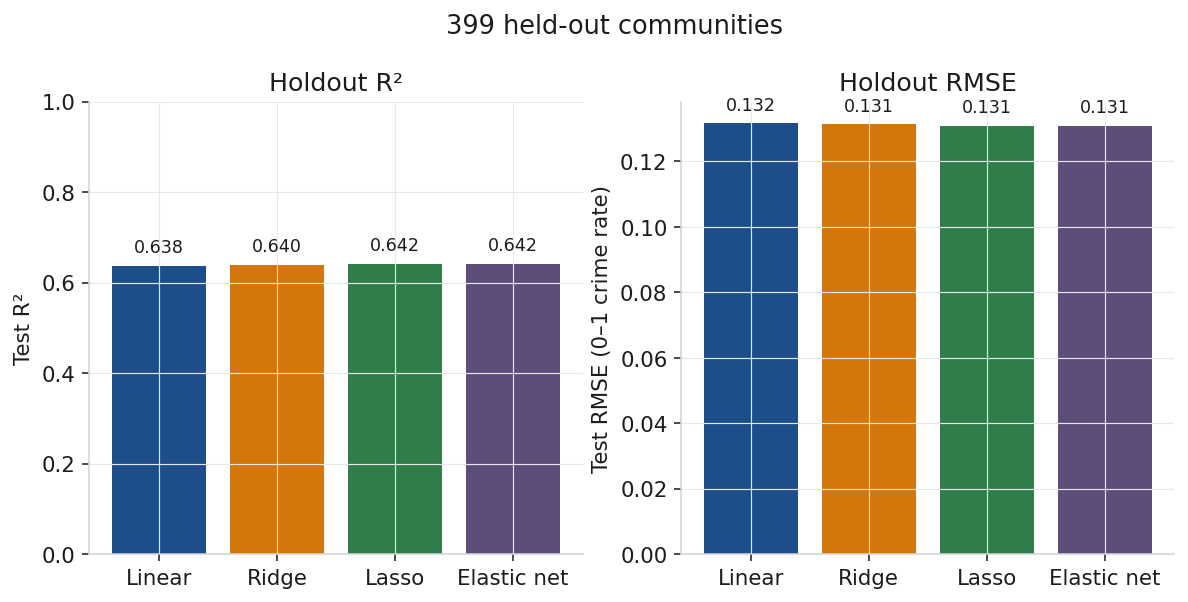
\includegraphics[width=\columnwidth]{06_holdout_metrics.png}
\caption{Holdout $R^{2}$ and RMSE for the 399 test communities on seed 42.}
\label{fig:holdout}
\end{figure}

\subsection{Five splits}
Table~\ref{tab:splits} is the check we cared about after seeing seed 42.
Ridge picks $\alpha=46.4$ on every seed.
The lasso picks $\alpha=0.001$ and keeps between 47 and 55 features.
On seed 42 that coarser lasso still has test $R^{2}$ 0.6422, next to 0.6421 on the fine grid, so the grid change is not driving the score.

Elastic net picks $\rho=0.1$ on four seeds and $\rho=0.5$ on seed 7.
The alpha on those runs ranges from 0.001 to 0.01, and the number of nonzero weights ranges from 47 to 82.
It is the best model on none of the five seeds.
The means are 0.6515, 0.6541, 0.6524, and 0.6523.
Ridge is ahead by about 0.003.
The standard deviation across seeds is about 0.03, roughly ten times the gap.
Mean test RMSE is 0.1351, 0.1346, 0.1349, and 0.1349.
If we had published only seed 42, we would have said the lasso won.
The average says ridge.
We do not think either sentence is a finding about accuracy.

\begin{table}[t]
\caption{Test $R^{2}$ when the split changes and the penalty is chosen again on that training set.}
\label{tab:splits}
\centering
\scriptsize
\begin{tabular}{@{}lcccc@{}}
\toprule
Seed & Linear & Ridge & Lasso & Elastic net \\
\midrule
0  & 0.6588 & 0.6583 & 0.6512 & 0.6501 \\
1  & 0.6091 & 0.6110 & 0.6125 & 0.6113 \\
7  & 0.6749 & 0.6806 & 0.6789 & 0.6780 \\
21 & 0.6768 & 0.6807 & 0.6771 & 0.6804 \\
42 & 0.6379 & 0.6400 & 0.6422 & 0.6417 \\
\midrule
Mean & 0.6515 & 0.6541 & 0.6524 & 0.6523 \\
\bottomrule
\end{tabular}
\end{table}

\section{Coefficients}
The accuracy comparison is flat.
The weights are not.
Table~\ref{tab:coef} takes columns where least squares is extreme and puts the penalized weights beside them.
A coefficient is the change in the normalized crime rate linked to a one-standard-deviation change in that column, with the other included columns held fixed in the equation.
Fig.~\ref{fig:coef} is the same comparison as a chart.

\begin{table}[t]
\caption{Standardized coefficients. A zero means that penalty dropped the column.}
\label{tab:coef}
\centering
\scriptsize
\begin{tabular}{@{}lrrrr@{}}
\toprule
Feature & Linear & Ridge & Lasso & Elastic net \\
\midrule
\texttt{PctRecImmig8}   & $+0.128$ & $+0.015$ & $+0.011$ & $+0.019$ \\
\texttt{PctRecImmig10}  & $-0.080$ & $+0.006$ & $0$      & $0$ \\
\texttt{TotalPctDiv}    & $-0.128$ & $-0.001$ & $0$      & $0$ \\
\texttt{MalePctDivorce} & $+0.093$ & $+0.028$ & $+0.030$ & $+0.031$ \\
\texttt{racepctblack}   & $+0.051$ & $+0.041$ & $+0.049$ & $+0.048$ \\
\bottomrule
\end{tabular}
\end{table}

\texttt{PctRecImmig8} and \texttt{PctRecImmig10} correlate at 0.996.
Least squares gives them $+0.128$ and $-0.080$.
Those two columns are almost the same measurement at two windows, eight years and ten.
The fit is using one to cancel the other.
Ridge pulls both weights in.
The lasso and elastic net keep a small positive weight on the eight-year column and drop the ten-year column.

\texttt{TotalPctDiv} correlates at $+0.55$ with the crime rate, the same direction as \texttt{MalePctDivorce}.
Least squares assigns it $-0.128$.
Once the other divorce columns are in the model, this extra copy is free to take a nonsense sign, and the infinite VIF is the same fact in another form.
Ridge moves the weight to about zero.
The lasso and elastic net drop the column.
\texttt{MalePctDivorce} stays positive under all four fits, which lines up with the raw correlation.

We are willing to repeat the associations that show up both in the correlations and in the penalized fits.
Communities with more children in two-parent households, and communities with more households receiving investment income, have lower predicted rates in this file.
Communities with a higher share of births to unmarried parents, a higher Black population share, and a higher male divorce rate have higher predicted rates.
Poverty sits in the same cluster.
\texttt{PctPopUnderPov} correlates at $+0.52$ with the target, and the lasso weight is slightly negative once the overlapping columns are included.
We read that as shared variance among the columns.
We would not write a sentence that says poverty lowers crime.

\begin{figure}[t]
\centering
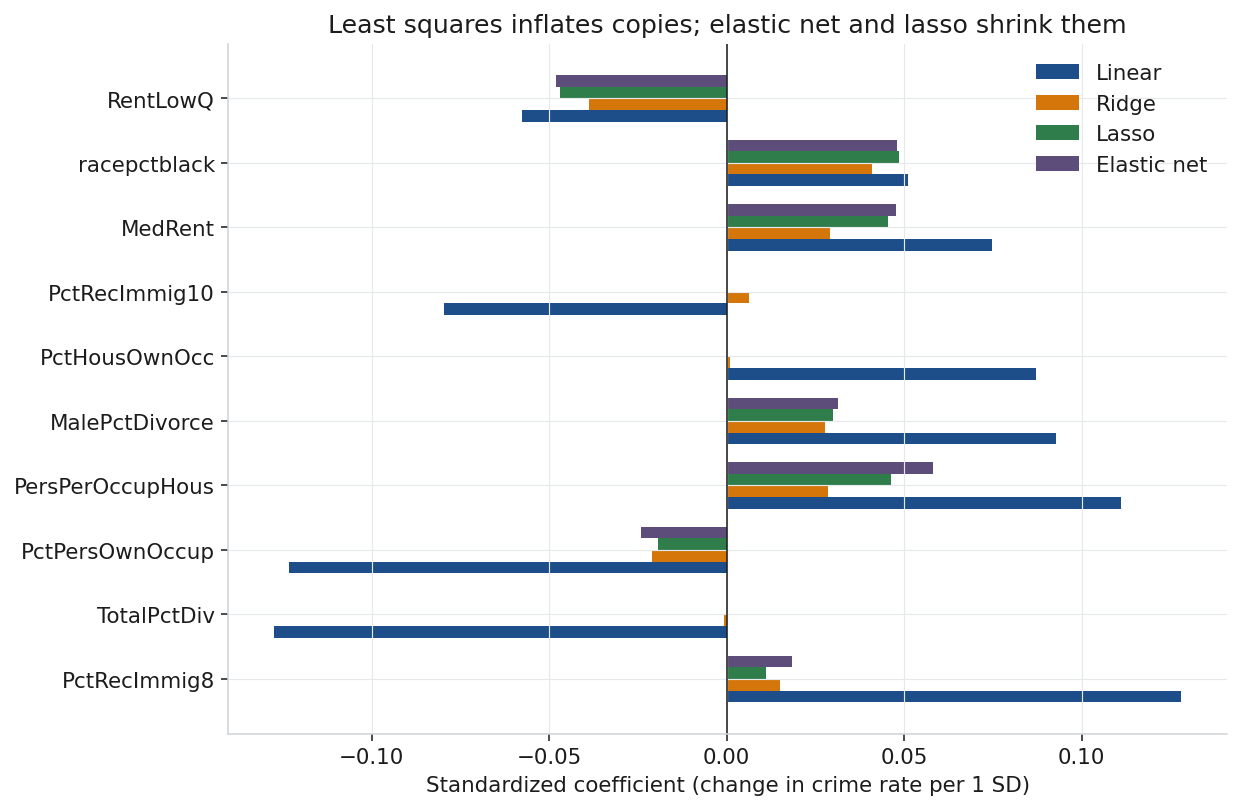
\includegraphics[width=\columnwidth]{09_coefficients.png}
\caption{The long bars are least squares on columns that are nearly duplicated. Ridge, the lasso, and elastic net pull those bars in.}
\label{fig:coef}
\end{figure}

\section{What we would and would not conclude}
We expected elastic net to land between ridge and the lasso, because that is how the method is usually described.
On this training set the cross-validation choice is $\rho=0.1$ and 81 nonzero weights.
The fit is a ridge-like penalty that also deletes some copies.
Calling it a third predictive model, without giving $\rho$, would oversell it.
Across the five splits it never has the lowest error.

The same restraint applies when a short lasso equation is offered as the structural account of violent crime \cite{dai2024,wei2025}.
The signs that match the raw correlations are worth showing.
They are partial associations after the other columns in the equation are held fixed.
They are not the change in crime we would see if a city changed one column.
Race shares are easy to over-read here.
They move with poverty, family structure, and housing, and our design does not separate those groups of columns.
Wei drops the race columns in order to look at the structural ones \cite{wei2025}.
That is a different question.
We kept them so the collinearity would stay visible.

The years also limit the claim.
The crime rate is from 1995 and most predictors are from the 1990 census.
We are not forecasting a later year, another country, or a patrol plan.
There are no interaction terms.
The wide residuals at high predicted crime are what that choice costs.
A nonlinear model might shrink the tail error.
We did not fit one, and a lower tail error would still not turn a coefficient into a cause.
The dropped LEMAS columns might matter for the departments that answered the survey.
A model for all 1{,}994 communities cannot use a field that is blank for about five communities out of six.

\section{Conclusion}
The census columns carry a real linear signal about the normalized violent-crime rate.
Using them cuts holdout RMSE by about two-fifths relative to the training mean, and the test $R^{2}$ is a bit over 0.60.
Least squares, ridge, the lasso, and elastic net are interchangeable if the only goal is that error.
On five splits the mean test $R^{2}$ values differ by about 0.003.
They are not interchangeable if the goal is a coefficient someone might quote.
Least squares puts large cancelling weights on near-duplicate columns, including a negative weight on a divorce measure that is positively correlated with crime.
Ridge shrinks those weights.
The lasso keeps 75 columns on the main split.
Elastic net, with $\ell_1$ ratio 0.1, keeps 81 and drops the same unstable copies.
We would cite this paper for that distinction, and not for a claim that one penalty forecasts crime.

\section*{Acknowledgment}
The numbers come from the public UCI extract \cite{uci2009}.
We did not collect new community data.
A reader who reruns the comparison should use seed 42 for the main split, a 40-point log grid from $10^{-4}$ to $10^{2}$ for the primary penalties, and seeds 0, 1, 7, 21, and 42 with a 16-point grid for the repeated splits.

\bibliographystyle{IEEEtran}
\bibliography{references}

\end{document}
